\documentclass[11pt]{aghdpl}

% Lista wszystkich języków stanowiących języki pozycji bibliograficznych użytych w pracy.
% (Zgodnie z zasadami tworzenia bibliografii każda pozycja powinna zostać utworzona zgodnie z zasadami języka, w którym dana publikacja została napisana.)
\usepackage[english,polish]{babel}

% Użyj polskiego łamania wyrazów (zamiast domyślnego angielskiego).
\usepackage{polski}

% Greckie litery w tekscie (zamiast w formułach matematycznych)
\usepackage{textgreek}

%pseudokod
\usepackage{algorithm2e} 
\usepackage{algorithmic}

% Kilka wyrażeń matematycznych na raz
\usepackage{amsmath}

\usepackage[utf8]{inputenc}

% dodatkowe pakiety

\usepackage{mathtools}
\usepackage{amsfonts}
\usepackage{amsmath}
\usepackage{amsthm}

% podświetlanie kodu
\usepackage[utf8]{inputenc}
\usepackage{minted}
\setminted[]{
    linenos=true,
    breaklines
}
\usepackage{etoolbox}
\AtBeginEnvironment{quote}{\singlespacing\small}
% --- < ścieżki > ---
\usepackage{graphicx}
\graphicspath{{media/}}


% --- < bibliografia > ---

\usepackage[
style=numeric,
sorting=none,
%
% Zastosuj styl wpisu bibliograficznego właściwy językowi publikacji.
language=autobib,
autolang=other,
% Zapisuj datę dostępu do strony WWW w formacie RRRR-MM-DD.
% urldate=iso8601,
% Nie dodawaj numerów stron, na których występuje cytowanie.
backref=false,
% Podawaj ISBN.
isbn=true,
% Nie podawaj URL-i, o ile nie jest to konieczne.
url=false,
%
% Ustawienia związane z polskimi normami dla bibliografii.
maxbibnames=3,
% Jeżeli używamy BibTeXa:
backend=bibtex
]{biblatex}
\addbibresource{bibliografia.bib}

\usepackage[autostyle]{csquotes}
% Ponieważ `csquotes` nie posiada polskiego stylu, można skorzystać z mocno zbliżonego stylu chorwackiego.
\DeclareQuoteAlias{croatian}{polish}



% Nie wyświetlaj wybranych pól.
%\AtEveryBibitem{\clearfield{note}}

% Użyj czcionki kroju Courier.
\usepackage{courier}

% ------------------------
% --- < listingi > ---
\usepackage{listings}
\lstloadlanguages{TeX}

% --- < kolorowy tekst > ---
\usepackage[dvipsnames]{xcolor}

% --- < Małe przerwy w dużych liczbach > ---
\usepackage{siunitx}

\usepackage{amsmath}

% --- < Do wygenerowania listy równań > ---
\usepackage[notlof]{tocbibind}
\usepackage{tocloft}


\lstset{
	literate={ą}{{\k{a}}}1
           {ć}{{\'c}}1
           {ę}{{\k{e}}}1
           {ó}{{\'o}}1
           {ń}{{\'n}}1
           {ł}{{\l{}}}1
           {ś}{{\'s}}1
           {ź}{{\'z}}1
           {ż}{{\.z}}1
           {Ą}{{\k{A}}}1
           {Ć}{{\'C}}1
           {Ę}{{\k{E}}}1
           {Ó}{{\'O}}1
           {Ń}{{\'N}}1
           {Ł}{{\L{}}}1
           {Ś}{{\'S}}1
           {Ź}{{\'Z}}1
           {Ż}{{\.Z}}1,
	basicstyle=\footnotesize\ttfamily,
}

% ------------------------

\AtBeginDocument{
	\renewcommand{\tablename}{Tabela}
	\renewcommand{\figurename}{Rys.}
}

% ------------------------
% --- < tabele > ---

\usepackage{array}
\usepackage{tabularx}
\usepackage{multirow}
\usepackage{booktabs}
\usepackage{makecell}
\usepackage{graphicx}
\usepackage[flushleft]{threeparttable}

% defines the X column to use m (\parbox[c]) instead of p (`parbox[t]`)
\newcolumntype{C}[1]{>{\hsize=#1\hsize\centering\arraybackslash}X}


%---------------------------------------------------------------------------

\author{Alicja Zoń}
\shortauthor{A. Zoń}

\titlePL{Oprogramowanie do analizy tekstów oparte o algorytmy uczenia maszynowego}

\shorttitlePL{Oprogramowanie do analizy tekstów oparte o algorytmy uczenia maszynowego} % skrócona wersja tytułu jeśli jest bardzo długi

\thesistype{Praca inżynierska}

\supervisor{dr hab. inż. Tomasz Szumlak}

\degreeprogramme{Informatyka Stosowana}

\date{2019}

\department{}

\faculty{Wydział Fizyki i Informatyki Stosowanej}

\acknowledgements{}


\setlength{\cftsecnumwidth}{10mm}

%---------------------------------------------------------------------------
\setcounter{secnumdepth}{4}
\brokenpenalty=10000\relax

\begin{document}

\titlepages

% Ponowne zdefiniowanie stylu `plain`, aby usunąć numer strony z pierwszej strony spisu treści i poszczególnych rozdziałów.
\fancypagestyle{plain}
{
	% Usuń nagłówek i stopkę
	\fancyhf{}
	% Usuń linie.
	\renewcommand{\headrulewidth}{0pt}
	\renewcommand{\footrulewidth}{0pt}
}

\addtocontents{toc}{\protect\setcounter{tocdepth}{-1}}
\tableofcontents
\addtocontents{toc}{\protect\setcounter{tocdepth}{2}}
    \clearpage
\addcontentsline{toc}{chapter}{Bibliography}

\chapter{Wstęp}
\label{cha:wstep}

\section{Wprowadzenie}
\label{sec:wprowadzenie}
Istotną częścią naszego codziennego życia jest pozyskiwanie informacji, choć często bardziej interesujące od faktów bywają opinie. Wraz z dynamicznym rozwojem Web 2.0, czyli sieci socjalnej, nastawionej głównie na treści generowane przez użytkowników portali, zwiększa się potrzeba kategoryzacji tychże tekstów. Wiedza o tym, jaka jest publiczna opinia na temat jakiegoś produktu, osoby bądź miejsca może znacznie ulepszyć strategie biznesowe, polityczne i marketingowe. Manualne przetworzenie tak dużej ilości danych jest bardzo czasochłonne, stąd konieczność stosowania systemów do ich automatycznej analizy.

Celem tej pracy jest stworzenie rozwiązania do analizy opinii w krótkich tekstach. W założeniu program ma określać, czy dane zdanie ma wydźwięk pozytywny, negatywny, czy neutralny. Motywacją do zbadania tego właśnie tematu jest chęć praktycznego zastosowania uczenia maszynowego w dziedzinie, która cieszy się popularnością i daje duże możliwości rozwoju.  
\section{Zawartość pracy}
\label{sec:zawartosc}

\begin{itemize}
  \item \textbf{Rozdział 2:} zawiera opis poruszanego problemu wraz z nakreśleniem możliwych podejść do jego rozwiązania. Przedstawiono uzasadnienie wyboru konkretnego podejścia oraz aktualny stan badań w tej dziedzinie (tzw. \textit{state of the art}).
  \item \textbf{Rozdział 3:} przedstawiono w nim źródło, z którego zostały zaczerpnięte dane do uczenia. Opisany jest sposób reprezentacji danych i etykietowania zdań. 
  \item \textbf{Rozdział 4:} opisuje modele teoretycznie możliwe do zastosowania w badanym problemie. Przedstawiony jest krótki opis i analiza tych modeli oraz ostateczna postać wybranego modelu wraz z wzorami i uzasadnieniem, dlaczego najbardziej pasuje do problemu opisywanego w tej pracy.
  \item \textbf{Rozdział 5:} wymieniono w nim użyte technologie i narzędzia wraz z ich zaletami i uzasadnieniem wyboru. 
  \item \textbf{Rozdział 6:} opisuje implementację modelu z rozdziału czwartego. Przedstawiony jest również dobór parametrów wraz z porównaniem wyników dla różnych wartości, a także regularyzacja modelu i korzyści z niej płynące.
  \item \textbf{Rozdział 7:} przedstawione są tu wyniki najlepszego wytrenowanego modelu wraz z wykresami poszczególnych metryk i analizą jakości klasyfikacji.
  \item \textbf{Rozdział 8:} zawiera analizę konkretnych przypadków wraz z wynikiem ich dopasowania. Opisane są zarówno przykłady prawidłowych dopasowań, jak i błędy pierwszego i drugiego rodzaju.
  \item \textbf{Rozdział 9:} przedstawia krótką dyskusję dotyczącą napotkanych problemów. Przedstawiono również możliwości rozwoju programu. 
  \item \textbf{Rozdział 10:} wnioski z pracy w kontekście realizacji jej celu i możliwości dalszego wykorzystania uzyskanych wyników.
\end{itemize}

\section{Aspekt twórczy i badawczy w pracy}
\label{sec:tworczosc}

Rozdziały od szóstego do dziewiątego stanowią część twórczo-badawczą, która opracowuje metody naukowe przedstawione w części teoretycznej pracy. Kod programu będącego przedmiotem analizy w tej pracy został stworzony w oparciu o źródła wymienione w bibliografii.



\chapter{Opis problemu}
\label{cha:opis}

Badanie opinii i emocji w tekstach (\textit{ang. sentiment analysis}) jest zadaniem dość trudnym, gdyż nawet ludzie różnie odbierają wydźwięk tych samych zdań. Dlatego stworzenie precyzyjnego klasyfikatora wydźwięku tekstu to duże wyzwanie, zwłaszcza że w zdaniach istotne są nie tylko słowa, ale także ich kolejność i kontekst. 

Wydźwięk tekstów może być analizowany w różnych skalach, w tej pracy przyjęte zostało podejście najbardziej podstawowe, czyli wykrywanie biegunowości (\textit{ang. polarity detection}), będące klasyfikacją zdań na trzy grupy opinii: pozytywne, negatywne oraz neutralne. 

\section{Zastosowana metoda}
\label{sec:technika}
Istnieje wiele technik i algorytmów, których używa się do analizy wydźwięku tekstu. Można je podzielić na dwie główne grupy: techniki oparte na regułach (leksykonie) oraz podejścia automatyczne wykorzystujące uczenie maszynowe. 

Podejście regułowe polega na klasyfikowaniu tekstów na podstawie przygotowanego wcześniej słownika, który zawiera listę słów i wyrażeń oraz przypisany do nich wydźwięk\cite{techniques}. Jeśli tekst posiada więcej słów pozytywnych niż negatywnych, to opinia jest klasyfikowana jako pozytywna, w przeciwnym wypadku jako negatywna. Podejście to posiada jednak kilka istotnych wad: po pierwsze stworzenie leksykonu wydźwięku jest czasochłonne i wymaga manualnego zdefiniowania reguł, a po drugie kontekst słów w zdaniu nie jest brany pod uwagę. Zatem jeśli w słowniku słowu \textit{podoba} jest przypisana etykieta pozytywna, to zdanie \textit{To mi się nie podoba} zostanie zaklasyfikowane jako pozytywne pomimo negacji.  

Natomiast w podejściu opartym o algorytmy uczenia maszynowego budowany jest automatyczny klasyfikator, który, mając zestaw danych treningowych, uczy się kojarzyć zadany wejściowy tekst z przypisanym mu wyjściem wynikowym (etykietą)\cite{techniques}. Uczenie przebiera różną formę, w zależności od wybranego modelu i stopnia jego skomplikowania. 

Do rozwiązania opisywanego problemu wybrana została technika uczenia maszynowego, gdyż wymaga dużo mniejszego nakładu pracy, daje możliwość osiągnięcia znacznie lepszych wyników, a końcowy system ma większą uniwersalność i skalowalność.

\section{\textit{State of the art}}
\label{sec:stateoftheart}
Wraz z rozwojem głębokiego uczenia maszynowego (\textit{ang. deep learning}), coraz powszechniejsze stało się stosowanie go w analizie tekstów, czego dowodem są liczne publikacje w tej dziedzinie\cite{survey}. Powstawanie nowych modeli sieci neuronowych doprowadziło w ostatnich dziesięciu latach do dużego postępu w automatycznej analizie wydźwięku tekstu\cite{survey}, a równocześnie zwiększyła się popularność takich badań. 

Tworzone są modele analizujące teksty pod kątem ich ogólnego wydźwięku, na poziomie zdań, a także w oparciu o konkretne aspekty, gdyż jedno zdanie może oceniać dwie różne kwestie (np. \textit{Fabuła była ciekawa, ale obsada mi się nie podobała}.). Najnowsze badania oprócz analizy tego, czy tekst jest pozytywny, czy negatywny, skupiają się również na rozpoznawaniu różnych emocji (np. gniew czy smutek), a także na wykrywaniu sarkazmu i ironii\cite{survey}. 

Większość tych prac analizuje teksty w języku angielskim, natomiast w języku polskim nie przeprowadzono jak dotąd wielu badań na ten temat {\textendash} przykładowe publikacje warte uwagi to projekt OPTA\cite{opta} Zespołu Inżynierii Lingwistycznej Polskiej Akademii Nauk, a także prace zgłoszone do konkursu PolEval 2017\cite{poleval}, gdzie jednym z zadań było stworzenie modelu do analizy wydźwięku tekstu.  

\chapter{Dane uczące}
\label{cha:dane}

Dane wykorzystane do uczenia i testowania stworzonego modelu zostały zaczerpnięte ze zbioru Treebank Wydźwięku (\textit{ang.  Polish Sentiment Treebank})\cite{treebank} w wersji 2.0. Zbiór uczący zawiera 2200 zdań o różnym stopniu złożoności, natomiast zbiór testowy składa się z 350 zdań. 

\section{Rozkład zdań}
\label{sec:rozklad}

Do plików z danymi tekstowymi dołączone są pliki \textit{parents} przedstawiające rozbiór gramatyczny zdań za pomocą drzew składniowych. Każde słowo ma przypisanego rodzica, czyli węzeł nadrzędny, natomiast korzeń drzewa posiada etykietę 0. W tabeli 3.1 przedstawiono przykładowe zdanie ze zbioru uczącego. Jak widać, w tym przypadku korzeniem drzewa jest słowo \textit{działali}.

\begin{table}[H]
\centering
\resizebox{\textwidth}{!}{%
\begin{tabular}{|l|c|c|c|c|c|c|c|c|c|c|}
\hline
\textbf{Pozycja w zdaniu} & 1                   & 2                & 3                   & 4           & 5             & 6                 & 7           & 8               & 9             & 10         \\ \hline
\textbf{Słowo lub znak}   & \textit{Zatrzymani} & \textit{wczoraj} & \textit{przestępcy} & \textit{od} & \textit{roku} & \textit{działali} & \textit{na} & \textit{własną} & \textit{rękę} & \textit{.} \\ \hline
\textbf{Rodzic}           & 3                   & 1                & 6                   & 6           & 4             & 0                 & 6           & 9               & 7             & 6          \\ \hline
\end{tabular}%
}
\caption{Przykładowe zdanie z wykorzystanego zbioru danych wraz z przypisanymi rodzicami.}
\label{table:bf-sa}
\end{table}

Dzięki takiemu rozbiorowi semantycznemu możliwe jest przedstawienie kontekstu słów w zdaniu w sposób zrozumiały dla sieci neuronowej.


\section{Etykiety}
Zdania w zbiorze danych są opatrzone etykietami wydźwięku (pliki \textit{labels}), gdzie \textit{-1} to opinia negatywna, \textit{0} \textendash \ neutralna, a \textit{1} pozytywna. Reprezentacja etykiet w zbiorze uczącym jest następująca: 54\% to etykiety pozytywne, natomiast 46\% \textendash \ negatywne. Ogólny wydźwięk zdania jest określany na podstawie etykiety korzenia drzewa, a także jego poddrzew. Jak widać na rys. 3.2, zdanie \textit{Widzę niepochlebne opinie o obsłudze, z którymi absolutnie się nie zgadzam.} zawiera człon \textit{widzę niepochlebne opinie o obsłudze}, który ma wydźwięk negatywny, dlatego został opatrzony etykietą \textit{-1}. Jednak negacja dalszej części zdania zmienia jego wydźwięk na pozytywny, dlatego korzeń drzewa ma ostetcznie etykietę \textit{1}. 
\label{sec:etykiety}
\begin{figure}[H]
    \centering
    \resizebox{\textwidth}{!}{%
    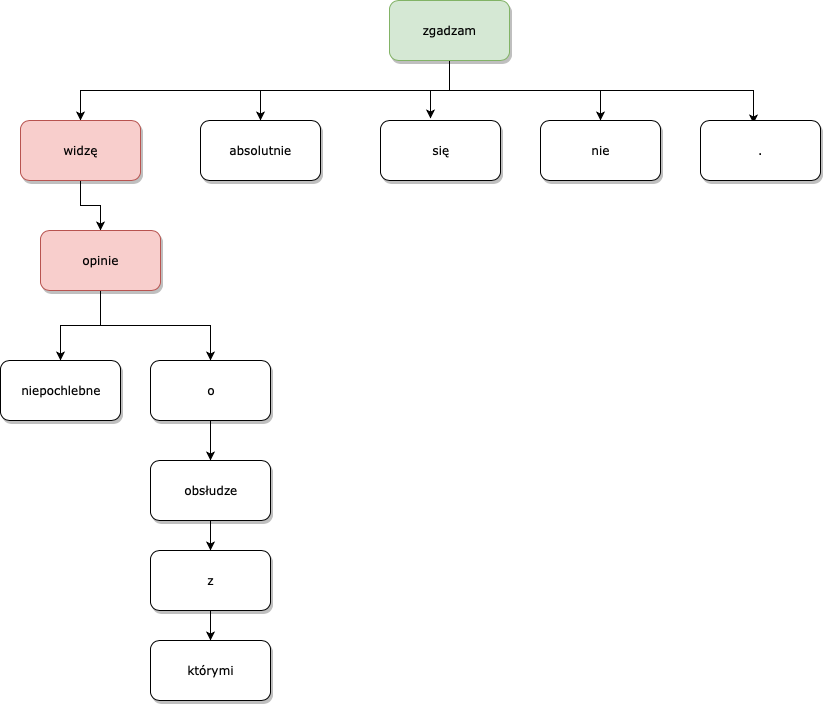
\includegraphics[clip]{labeled-tree.png}
    }%
    \caption{Drzewo zdania wraz z etykietami wydźwięku dla każdego poddrzewa.}
\end{figure}



\chapter{Wybrany model}
\label{cha:model}

\section{Rekurencyjna sieć neuronowa}
\label{sec:rozklad}
 
Zdania to sekwencje danych, zatem warto jest wybrać taki algorytm, który podczas procesu uczenia zapamiętuje poprzednie elementy w sekwencji. Dzięki temu możliwe będzie wytrenowanie sieci w taki sposób, by kojarzyła dany wynik nie tylko z konkretnym słowem, ale także z pozostałymi słowami w zdaniu i ich kolejnością. 

Rekurencyjna sieć neuronowa (RNN) rozszerza połączoną sieć neuronową (wzór 4.1) tak, by aktualny stan  \textit{$h_t$}  był obliczany na podstawie akutalnego wejścia \textit{$x_t$} oraz poprzedniego stanu \textit{$h_{t-1}$}\cite{tai}. 
\begin{equation} y = \sigma(Wx) \end{equation} 
Najpopularniejszą postać RNN przedstawia wzór 4.2.
\begin{equation} h_t = tanh(W_x x_t + W_h h_{t-1}) \end{equation} 

Rozwiązanie to nie jest optymalne, gdyż w tego typu sieciach występuje problem znikającego lub ekspolodującego gradientu\cite{gradient}. Oznacza to, że podczas uczenia gradient może wykładniczo maleć bądź rosnąć. W pierwszym przypadku sieć coraz gorzej aktualizuje wagi (lub nawet przestaje je aktualizować), zatem nie jest w stanie wyuczyć się zależności występujących w dłuższych sekwecjach. Natomiast rezultatem zbyt dużego gradientu są znaczne zmiany w macierzach wag, co może skutkować tym, że model będzie przeskakiwał minima i nigdy ich nie osiągnie, a w skrajnych przypadkach wartość funkcji kosztu wyniesie NaN.

\section{LSTM}
\label{sec:lstm}

Problemowi znikającego gradientu zapobiega sieć LSTM\cite{tai} (\textit{ang. Long Short-Term Memory}), która wprowadza strukturę \textit{$c_t$} zwaną komórką pamięci, mającą możliwość przechowania informacji na przestrzeni czasu. Przepływ informacji z poprzednich stanów kontroluje mechanizm bramek: wejściowej \textit{$i_t$}, zapominającej \textit{$f_t$} oraz wyjściowej \textit{$o_t$}. Wzory 4.3 - 4.8 przedstawiają wariant sieci LSTM użyty w tej pracy, gdzie \textit{$W_x$} i \textit{$W_h$} to macierze wag.

\begin{equation} i_t = \sigma(W_{xi}x_t + W_{hi}h_{t-1} + b_i) \end{equation}
\begin{equation} f_t = \sigma(W_{xf}x_t + W_{hf}h_{t-1} + b_f) \end{equation}
\begin{equation} c_t = c_0 * f_t + i_t * tanh(W_{ci}x_t + W_{hc}h_{t-1} + b_c)  \end{equation}
\begin{equation} o_t = \sigma(W_{xo}x_t + W_{ho}h_{t-1} + b_o) \end{equation}
\begin{equation} c_0 = c_t \end{equation}
\begin{equation} h_t = o_t * tanh(c_0) \end{equation}

\section{Struktura drzewa w LSTM}
\label{sec:tree}

Ograniczeniem typowej architektury LSTM jest to, że pozwala ona tylko na sekwencyjną propagację informacji. Aby móc przetworzyć dane, które są przedstawione w postaci drzew zależności, konieczne jest wprowadzenie rozszerzonej sieci zwanej Tree-LSTM\cite{tai}. Od zwykłej sieci LSTM różni się tym, że aktualizacje wektorów bramek i komórki pamięci zależą nie od jednego stanu poprzedniego, ale od stanów wszystkich dzieci danego węzła.

Niniejsza praca opiera się na modelu zaproponowanym przez Michała Lwa i Piotra Pęzika\cite{treelstm}, który nosi nazwę \textit{Sequential Child-Combination Tree-LSTM}. Ma on taką samą postać jak model LSTM ze wzorów 4.3 - 4.8, z tą jednak różnicą, że aktualny stan \textit{$h_t$}  węzła jest wyliczany z kombinacji \textit{k} stanów jego dzieci. Zatem wartość komórki pamięci \textit{$c_{ik}$} jest wyznaczana korzystając ze stanu ukrytego \textit{$h_{ck}$} poprzedniego dziecka w sekwencji (dzieci są ułożone w kolejności występowania w zdaniu), co przedstawiają wzory 4.9 - 4.13. 

\begin{equation} c_{i1} = c_0 * f_{i1} + i_{i1} * tanh(W_{ci}x_t + W_{hc}h_{c1} + b_c)  \end{equation}
\begin{equation} c_{i2} = c_{i1} * f_{i2} + i_{i2} * tanh(W_{ci}h_{i1} + W_{hc}h_{c2} + b_c)  \end{equation}
\centerline {...}
\begin{equation} c_{in} = c_{in} * f_{in} + i_{in} * tanh(W_{ci}h_{in-1} + W_{hc}h_{cn} + b_c)  \end{equation}
\begin{equation} c_t = c_{in}  \end{equation}
\begin{equation} h_t = h_{in}  \end{equation}

\section{Wektorowa reprezentacja słów}
\label{sec:vector}

Do wektorowej reprezentacji słów w przestrzeni (\textit{ang. word embedding)} służy model \textit{Word2vec}. Przyporządkowuje on podobne słowa do punktów położonych blisko siebie w przestrzeni wektorowej\cite{word2vec}. 

Mapowanie odbywa się przy pomocy macierzy \textit{J}  o losowych wartościach i wymiarach  \textit{MxN}, gdzie \textit{M} to rozmiar słownika zawierającego wszystkie słowa z danych uczących, natomiast \textit{N} to przyjęty rozmiar macierzy (zazwyczaj przyjmuje się którąś z potęg liczby 2).   
\chapter{Wykorzystane narzędzia i technologie}
\label{cha:technologie}

\section{Python 3.5}
\label{sec:python}
Python jest najpopularniejszym językiem programowania w uczeniu maszynowym \textendash \ według raportu firmy Vision Mobile\cite{visionmobile} używa go 57\% programistów i naukowców związanych z przetwarzaniem danych. Na kolejnych miejscach znajduje się C/C++ (używany przez 43\% programistów) oraz Java (41\%). 

Powyższy raport przytacza również konkretne najpopularniejsze obszary zastosowań danych języków. Język Python jest najbardziej powszechny w eksploracji danych z sieci (\textit{ang. web mining}), przetwarzaniu języka naturalnego oraz w analizie wydźwięku tekstu (używany przez 44\% programistów). Dzieje się tak dlatego, że Python to język o przejrzystej składni, kładący nacisk na prostotę i czytelność\cite{python}. Zaletą są również liczne biblioteki, które można wykorzystać do uczenia maszynowego, między innymi PyTorch, TensorFlow, SciKit i Pandas.

\section{TensorFlow}
\label{sec:tensorflow}

Tensorflow to biblioteka powszechnie wykorzystywana w głębokim uczeniu maszynowym. Dużą zaletą jest możliwość stworzenia całej sieci za pomocą zmiennych zastępczych (\textit{ang. placeholder}). Umożliwiają one oddzielenie fazy konfiguracji od fazy ewaluacji, co pozwala na łatwe skalowanie sieci. Biblioteka ta jest niskopoziomowa, ma więc dużo możliwości do dostosowywania sieci do konkretnych potrzeb. 
Posiada również szczegółową dokumentację z przykładami immplementacji\cite{tensorflow}, a z racji dużej popularności, łatwo znaleźć wiele źródeł i tutoriali wykorzystujących TensorFlow.

Przed przystąpieniem do implementacji brana była pod uwagę również biblioteka Keras. Zapewnia ona wysokopoziomowy interfejs programowania aplikacji, co sprawia, że stworzenie sieci LSTM jest proste i nie wymaga wiele kodu. Ograniczona możliwość dostosowania poszczególnych parametrów sieci sprawia jednak, że w opisywanym w tej pracy przypadku użycie biblioteki Keras się nie sprawdza. 

\section{Scikit-learn}
\label{sec:scikit}

Jest to biblioteka przeznaczona do uczenia maszynowego. W pracy został wykorzystany jej moduł \textit{metrics}\cite{scikit}. Posiada on liczne funkcje do ewaluacji modelu oraz mierzenia jakości klasyfikacji. Na stronie biblioteki opisane są również przykłady zastosowania każdej z metryk oraz sposób interpretacji otrzymanych wyników.

\section{Pozostałe narzędzia}
\label{sec:pozostale}
\begin{itemize}
  \item \textbf{NumPy} \textendash \ biblioteka służąca do obliczeń numerycznych.
  \item \textbf{Pyplot} \textendash \ moduł biblioteki Matplotlib służący do sporządzania wykresów.
\end{itemize}



\chapter{Implementacja}
\label{cha:implementacja}

\section{Przygotowanie danych}
\label{cha:przygotowanie}

Przygotowany został moduł \textit{data}, w którym dane są wczytywane i poddawane obróbce koniecznej do przeprowadzenia prawidłowego procesu uczenia. 

Każde słowo ze zbioru danych zapisano do słownika \textit{word2idx} i przypisano mu unikalny indeks. W celu przyspieszenia działania programu zamieniono wszystkie słowa w zdaniach na ich indeksy ze słownika. 

Lista etykiet określających rodziców została zastąpiona słownikiem, w którym kluczami są kolejne węzły, a wartościami \textendash \ lista ich dzieci lub pusta lista w przypadku braku dzieci. 

\section{Implementacja modelu}
\label{cha:implementacjamodelu}

Mamy trzy sekwencje, po których potrzebujemy przeiterować w tym samym czasie: listę słów, która zawierającą indeksy ze słownika \textit{word2idx}, listę dzieci poszczególnych węzłów oraz listę etykiet ich wydźwięku. Potrzebna jest zatem pętla, która przejdzie przez te sekwencje. Nie znane są jednak na tym etapie wartości tych zmiennych, ani nawet ich długości, nie można więc użyć zwykłej pętli \textit{while}. Wykorzystano w tym przypadku \textit{tf.while\_loop} z biblioteki TensorFlow (listing 1), która powtarza funkcję \textit{pętla} dopóki \textit{warunek} jest prawdziwy. 

\begin{listing}[]
\lstinputlisting[language=python]{listing/while.py}
\caption{Pętla generująca tablicę wyjść.}
\end{listing}

Warunkiem zakończenia pętli jest tutaj koniec zdania, natomiast ciało wykonywanej funkcji przedstawia listing 2. Dla każdego dziecka danego węzła obliczane są wartości poszczególnych bramek LSTM według wzorów podanych w rozdziale czwartym. W momencie gdy algorytm dojdzie do korzenia drzewa, który znajduje się na końcu listy, przeprowadzane jest mapowanie słowa na wektor liczb rzeczywistych. 
\\

\begin{listing}[]
\begin{algorithmic}
\FOR{dziecko \textbf{in} lista dzieci} 
\IF {węzeł nie jest korzeniem} 
        \STATE $h_1 = oblicz\_bramki(h_1, wyjscie(dziecko))$
\ELSE
        \STATE $h_1 = mapuj(aktualne\ slowo)$
        \ENDIF
\ENDFOR
\end{algorithmic}
\caption{Funkcja wyznaczająca stan aktualnego węzła.}
\end{listing}

Po zakończeniu pętli otrzymujemy ostateczną wyjściową tablicę. Mnożona jest ona przez wyjściową macierz wag i wyjściowy bias. Otrzymany wynik wykorzystywany jest do wyznaczenia wartości funkcji kosztu. W programie użyta została funkcja \textit{sparse\_softmax\_cross\_entropy\_with\_logits}, którą stosuje się do problemów klasyfikacji wieloklasowej. 

Zasadniczo cała implementacja sprowadza się do następujących etapów:
\begin{itemize}
  \item Wczytanie danych
  \item Zbudowanie modelu LSTM
  \item Wyznaczenie wartości kosztu
  \item Uruchomienie pętli uczenia
  \item Wyświetlenie wyników
 \end{itemize}


\section{Dobór parametrów}
\label{cha:parametry}

\subsection{Wybór optymalizatora}
Optymalizator to algorytm mający na celu znalezienie minimum zadanej funkcji kosztu. Wybór metody optymalizacji używanej w procesie uczenia miał duży wpływ na otrzymywane wyniki, co widać w tabeli 6.1. Zbadano optymalizator gradientu prostego, a także jego modyfikacje: \textit{Momentum}, \textit{Adagrad} oraz \textit{Adam}. Powodem wybrania tych czterech algorytmów do analizy był fakt, że powtarzały się one najczęściej w znalezionych przykładach implementacji róznych modeli LSTM. 

W każdym przypadku rozmiar partii wynosił 32, natomiast wartość wskaźnika uczenia \textendash \ 0.01. W tabeli 6.1 widać bardzo dużą różnicę między wynikami osiąganymi przez optymalizator Adam, a pozostałymi algorytmami. Nie ma więc wątpliwości, że Adam najlepiej sprawdzi się w trenowaniu zaporojektowanej tutaj sieci.

\begin{table}[H]
\centering
\begin{tabular}{|l|c|c|c|c|}
\hline
\textbf{Klasyfikator}           & Adam             & Adagrad         & Gradient prosty              & Momentum         \\ \hline
\textbf{Dokładność uczenia}     & \textbf{96,78\%} & 77,3\% & 89,47\% & 86,59\% \\ \hline
\textbf{Wartość funkcji kosztu} & \textbf{2.56}           & 11,12         & 5,2            & 4,58           \\ \hline
\end{tabular}%

\caption{Porównanie wyników po 10 epokach uczenia.}
\label{table:bf-sa}
\end{table}

\subsection{Wskaźnik uczenia}

Wskaźnik uczenia (\textit{ang. learning rate}) wpływa na to, jak szybko aktualizowane są wagi \textendash \ zbyt wysoka wartość sprawia, że sieć może przeskakiwać minima, natomiast zbyt niska znacznie wydłuża czas uczenia. Tabela 6.2 przedstawia porównanie wyników dla 32-wymiarowej warstwy ukrytej i optymalizatora Adam. Jak widać, wysoki wskaźnik uczenia się nie sprawdza. W bibliotece TensorFlow dla optymalizatora Adam domyślnym wskaźnikiem uczenia jest wartość 0,001, jednak w opisywanym tutaj przypadku lepiej sprawdza się wartość 0,01, gdyż osiąga dobre wyniki w rozsądnym czasie. 

\begin{table}[H]
\centering

\begin{tabular}{|l|c|c|c|}
\hline
\textbf{Wskaźnik uczenia}       & 0,1     & 0,01    & 0,001   \\ \hline
\textbf{Dokładność uczenia}     & 77,25\% & \textbf{96,78\%} & 96,64\% \\ \hline
\textbf{Wartość funkcji kosztu} & 12.05 & \textbf{2.56}  & 4.31  \\ \hline
\end{tabular}%

\caption{Porównanie wyników po 10 epokach uczenia.}
\label{table:bf-sa}
\end{table}

\subsection{Wymiary warstwy ukrytej}

Działanie modelu zostało sprawdzone dla różnych wymiarów warstwy ukrytej. W każdym przypadku użyty został optymalizator Adam, natomiast wskaźnik uczenia wynosił 0.01. Jak widać w tabeli 6.2, wartości w zakresie 8-32 dają bardzo zbliżone wyniki w kwestii dokładności uczenia i wartości funkcji kosztu, z niewielką przewagą 32-wymiarowej warstwy ukrytej.

W literaturze nie znaleziono uzasadnienia wpływu tego parametru na ostateczne wyniki, można więc uznać dobór wymiarów warstwy ukrytej za kwestię indywidualną. Im większa jest ta wartość, tym dłuższy jest czas obliczeń: przy 16 wymiarach czas obliczeń jednej epoki wynosił 150 s, przy 32 \textendash \ 200 s, natomiast dla 64-wymiarowego stanu ukrytego już 337 s.
\begin{table}[H]
\centering
\begin{tabular}{|l|c|c|c|c|l|}
\hline
\textbf{Wymiary warstwy ukrytej}         & 4       & 8       & 16      & 32      & 64  \\ \hline
\textbf{Dokładność uczenia}     & 95,46\% & 97,02\% & 96,93\% & \textbf{97,09\%} & 96,44\% \\ \hline
\textbf{Wartość funkcji kosztu} & 3.55  & 2.39  & 2.3   & \textbf{2.25}  & 2.55\% \\ \hline
\end{tabular}%

\caption{Porównanie wyników po 15 epokach uczenia.}
\label{table:bf-sa}
\end{table}

\section{Regularyzacja modelu}


\label{cha:regulacja}
\subsection{Regularyzacja funkcji kosztu}
W celu zwiększenia wydajności modelu i uniknięcia przeuczenia (nadmiernego dopasowania) stosuje się różne techinki regularyzacji. Jedną z typowych metod jest regularyzacja l2, która polega na wyznaczeniu regularyzacyjnej funkcji kosztu będącej sumą normy $L^2$ obliczonej dla wag wejściowych \textit{$W_{xi}$} oraz dla wag wyjściowych \textit{U}, co przedstawia wzór 6.1. Wartość 0,02 jest tu dobranym parametrem optymalnym do używanego modelu. Wyznaczenie całkowitego kosztu polega na zsumowaniu wartości funkcji kosztu i wartości funkcji regularyzacji.

\begin{equation}
r = 0,02 * L^2(W_{xi}) + L^2(U) \end{equation}

\subsection{Wpływ wag na proces uczenia}
Samo zaincjalizowanie macierzy wag losowymi wartościami może doprowadzić do problemu znikającego lub eksplodującego gradientu, który został opisany w rozdziale 4. Aby temu zapobiec, wartości początkowe macierzy wyznaczono za pomocą heurystyki ze wzoru 6.1.
\begin{equation}
W = random(M, N) * \sqrt{\frac{1}{M+N}}
\end{equation}


\label{sec:etykiety}
\begin{figure}[H]
    \centering
    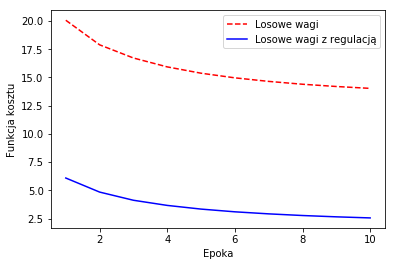
\includegraphics[clip]{weight_regulation.png}
    \caption{Porównanie wyników dla macierzy wag inicjalizowanych losowo oraz losowo z regularyzacją.}
\end{figure}
Na wykresie 6.1 widać jak dużą wpływ na osiąganą wartość funkcji kosztu ma zastosowanie powyższej regularyzacji.

Ciekawym eksperymentem okazało się również zmniejszenie wag poprzez pomnożenie każdej macierzy przez parametr o wartości 0,05. Jak widać na wykresie 6.2, nie wprowadza to znacznych zmian, choć to ulepszenie pozwala na osiągnięcie danej wartości funkcji kosztu o dwie epoki szybciej niż w przypadku, gdy nie mnożymy macierzy przez parametr. 

\label{sec:etykiety}
\begin{figure}[H]
    \centering
    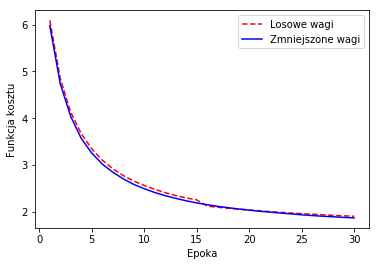
\includegraphics[clip]{min_weights.png}
    \caption{Porównanie wyników dla macierzy wag inicjalizowanych losowo oraz losowo ze zmniejszonymi wagami.}
\end{figure}



\chapter{Metryki}
\label{cha:metryki}
Podstawowymi miarami obrazującymi jakość uczenia sieci neuronowej jest dokładność (\textit{ang. accuracy}) oraz wartość funkcji kosztu (\textit{ang. loss value}).

Dokładność to procent prawidłowych klasyfikacji, zatem wyznaczenie tej wartości dla zbioru uczącego i testowego obrazuje jakość uczenia. Można również zaobserwować, czy jest różnica między tym, jak sieć radzi sobie z danymi, które już zna i tymi, które widzi po raz pierwszy.

Celem procesu uczenia jest minimalizacja funkcji kosztu, zatem im niższa jej wartość, tym lepsza jest nasza sieć. Gdy wartość tej funkcji zaczyna rosnąć, mamy do czynienia z problemem przeuczenia.

\section{Porównanie metryk}
\label{cha:wyniki}
Pierwszy analizowany model ma następujące parametry:
\begin{itemize}
  \item Optymalizator: \textbf{Adam}
  \item Wskaźnik uczenia: \textbf{0,01}
  \item Wymiary warstwy ukrytej: \textbf{16}
  \item Liczba epok: \textbf{20}
 \end{itemize}
 
 Jak widać na wykresie 7.1, występuje duża rozbieżność między dokładnością zbioru uczącego a dokładnością zbioru treningowego i testowego. W każdym z analizowanych podczas badań przypadków ta różnica była podobna lub nawet większa. Ani razu podczas przeprowadzanych badań nie udało się osiągnąć w zbiorze testowym dokładności większej niż 78\%.m. Powodem takiej sytuacji może być zjawisko nadmiernego dopasowania, gdzie model uczy się konkretnych reguł, których nie jest w stanie rozszerzyć poza zbiór uczący. Iną przyczyną może być zbyt mała ilość danych uczących. Ta opcja jest bardziej prawdopodobna, gdyż dokładność w zbiorze testowym stabilizuje się już po kilku epokach i ma bardzo zbliżone wartości niezależnie od wyboru parametrów (dlatego w rozdziale szóstym wartość ta nie została uwzględniona w tabelach porównawczych). Końcowa dokładność klasyfikacji zbioru uczącego to 96,77\%, jest to również wartość nalepsza ze wszystkich epok. Dla zbioru testowego dokładność po dwudziestu epokach wynosi 76,6\%, natomiast najlepszą wartość wynoszącą 78\% uzyskano w ósmej epoce.
 
 \label{sec:etykiety}
\begin{figure}[H]
    \centering
    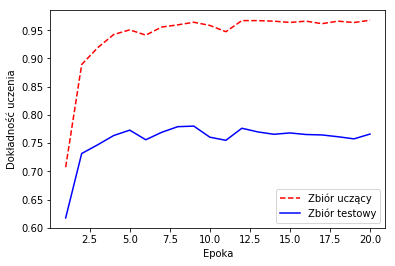
\includegraphics[clip]{accuracy16.png}
    \caption{Porównanie dokładności uczenia dla zbioru treningowego i testowego.}
\end{figure}


 \label{sec:etykiety}
\begin{figure}[H]
    \centering
    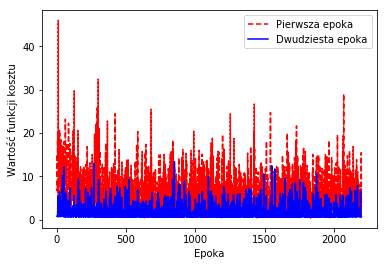
\includegraphics[clip]{compare-loss16.png}
    \caption{Porównanie wartości funkcji kosztu dla pierwszej i dwudziestej epoki uczenia.}
\end{figure}

Wykres 7.2 obrazuje różnicę w wartościach funkcji kosztu osiąganych w pierwszej i ostatniej epoce treningu. Widzimy, że proces uczenia przebiega prawidłowo \textendash \ średni koszt w pierwszej epoce wynosi 6,12, natomiast w dwudziestej 1,63. 

Wartość funkcji kosztu dla danych testowych szybko się stabilizuje osiągając minimum, co pokazuje wykres 7.3. Średni koszt w ostatniej epoce wynosi 0,69. 

 \label{sec:etykiety}
\begin{figure}[H]
    \centering
    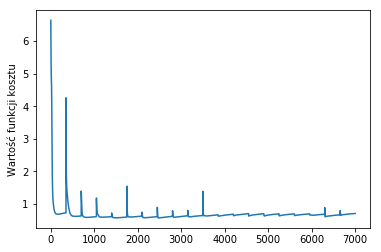
\includegraphics[clip]{test-loss16.png}
    \caption{Wartość funkcji kosztu dla zbioru testowego.}
\end{figure}

Dla porównania przeanalizowano również wykresy modelu z następującymi parametrami:
\begin{itemize}
  \item Optymalizator: \textbf{Adam}
  \item Wskaźnik uczenia: \textbf{0,01}
  \item Wymiary warstwy ukrytej: \textbf{32}
  \item Liczba epok: \textbf{70}
 \end{itemize}
 
 Jak widać na wykresie 7.4, dokładność klasyfikacji zbioru uczącego osiąga stabilność po ósmej epoce, a wartości są zbliżone do tych z wykresu 7.1. Wynik uzyskany po siedemdziesięciu epokach to 96,8\%, natomiast najlepsza uzyskana wartość to 97,8\%. 
 
  \label{sec:etykiety}
\begin{figure}[H]
    \centering
    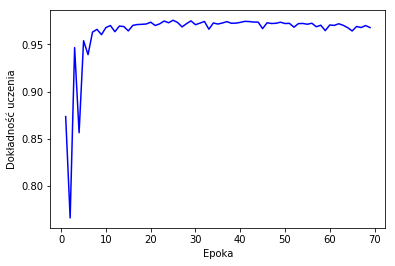
\includegraphics[clip]{train_acc.png}
    \caption{Dokładność uczenia dla zbioru treningowego.}
\end{figure}

 \label{sec:etykiety}
\begin{figure}[H]
    \centering
    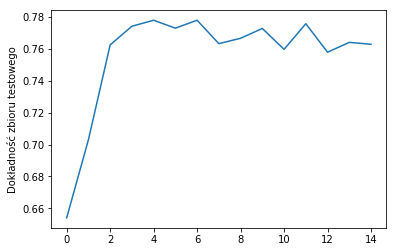
\includegraphics[clip]{test_acc.png}
    \caption{Dokładność uczenia dla zbioru testowego.}
\end{figure}

Dokładność dopasowań w zbiorze testowym (wykres 7.5) po siedemdziesięciu epokach wynosi 76,4\%, natomiast najlepsza uzyskana to 77,79\%. 

Zastanawiający jest przebieg wykresu 7.6, przedstawiającego zmianę wartości funkcji kosztu dla danych testowych. Wartość ta rośnie w miarę uczenia, co wskazuje na to, że mamy do czynienia z przeuczeniem. Jednak na wykresie 7.5 widzimy, że dokładność uczenia wraz z kolejnymi epokami utrzymuje się na tym samym poziomie. Może to oznaczać, że mimo iż model nie popełnia nowych błędów, to coraz bardziej utwierdza się w błędnych dopasowaniach.


 \label{sec:etykiety}
\begin{figure}[H]
    \centering
    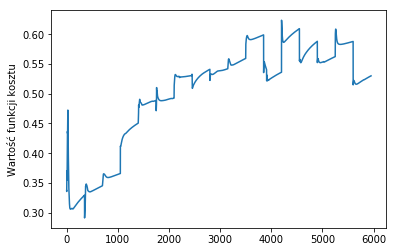
\includegraphics[clip]{test_loss.png}
    \caption{Wartość funkcji kosztu dla zbioru testowego.}
\end{figure}

Dla zbioru uczącego wartość funkcji kosztu w ostatniej epoce jest znacznie niższa niż w siedemdziesiątej (co przedstawia wykres 7.7), więc w tym przypadku sieć zachowuje się prawidłowo.

Do dalszej analizy metryk w tym rozdziale oraz przypadków w rozdziale 8 wybrano drugą z opisywanych w tym podpunkcie sieci.

 \label{sec:etykiety}
\begin{figure}[H]
    \centering
    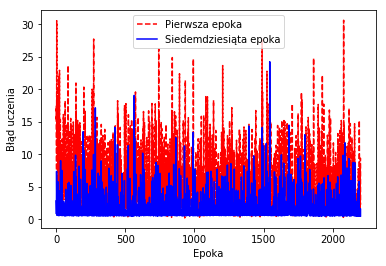
\includegraphics[clip]{epoch1vs70.png}
    \caption{Porównanie wartości funkcji kosztu dla pierwszej i siedemdziesiątej epoki uczenia.}
\end{figure}
 
\section{Raport klasyfikacji}
\label{cha:wyniki}

\begin{table}[H]
\centering
\begin{tabular}{|lllll|}
\hline
\multicolumn{1}{|l|}{\textbf{}}               & \multicolumn{1}{c|}{\textbf{precyzja}} & \multicolumn{1}{c|}{\textbf{czułość}} & \multicolumn{1}{l|}{\textbf{miara F-1}} & \textbf{liczba wystąpień} \\ \hline
\multicolumn{1}{|l|}{\textbf{neutralne}}      & \multicolumn{1}{c|}{0,84}              & \multicolumn{1}{c|}{0,90}         & \multicolumn{1}{l|}{0,87}               & 3666                      \\ \hline
\multicolumn{1}{|l|}{\textbf{pozytywne}}      & \multicolumn{1}{c|}{0.70}              & \multicolumn{1}{c|}{0,40}         & \multicolumn{1}{l|}{0,51}               & 1016                      \\ \hline
\multicolumn{1}{|l|}{\textbf{negatywne}}      & \multicolumn{1}{c|}{0,29}              & \multicolumn{1}{l|}{0,41}         & \multicolumn{1}{l|}{0,34}               & 365                       \\ \hline
\end{tabular}
\caption{Raport klasyfikacji modelu po 70 epokach uczenia.}
\label{table:bf-sa}
\end{table}

Precyzja to stosunek liczby prawdziwie pozytywnych dopasowań do wszystkich dopasowań. Jak widać sieć radzi sobie dobrze z dopasowaniem etykiet neutralnych i całkiem dobrze rozpoznaje wydźwięk pozytywny. Natomiast w przypadku etykiet negatywnych mamy bardzo niską precyzję, widać, że w większości przypadków sieć źle dopasowuje wydźwięk negatywny.

Czułość to stosunek liczby dopasowań prawdziwie pozytywnych do ogólnej liczby możliwych dopasowań. W tym przypadku widzimy, że tylko 40\% etykiet pozytywnych zostało dopasowanych. 

Miara F-1 jest średnią harmoniczną precyzji i czułości, zatem obrazuje ogólną jakość modelu. Widzimy, że dla etykiet neutralnych klasyfikacja przebiega prawidłowo, natomiast dla etykiet pozytywnych i negatywnych nie działa zbyt dobrze. 

Powodem takich wyników może być znaczna przewaga etykiet neutralnych w zbiorze uczącym, dzięki czemu sieć mogła się lepiej wyuczyć związanych z nimi zależności. Najmniej liczne były etykiety negatywne, co przekłada się na wyniki klasyfikacji. Dokładną liczbę dopasowań konkretnych etykiet do danych testowych obrazuje macierz konfuzji z rys. 7.8.


\label{sec:etykiety}
\begin{figure}[H]
    \centering
    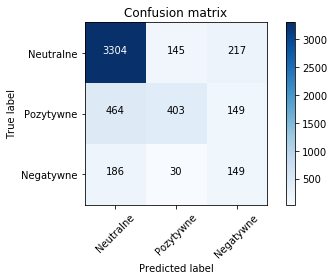
\includegraphics[clip]{conmat67.png}
    \caption{Macierz konfuzji modelu po 70 epokach uczenia.}
\end{figure}



\chapter{Analiza przypadków}
\label{cha:analiza}

\section{Prawidłowe dopasowania}
\label{cha:prawidlowe}

W zbiorze testowym znajdują się zdania o różnym stopniu skomplikowania. Na początek do analizy wybrano proste zdanie o pozytywnym wydźwięku:
\begin{table}[H]
\centering
\begin{tabular}{|l|c|c|l|c|}
\hline
\textbf{Zdanie}                & \textit{Flakon} & \textit{dość} & \textit{ładny} & \textit{.} \\ \hline
\textbf{Etykiety rzeczywiste}  & 0               & 0             & 1              & 0          \\ \hline
\textbf{Etykiety przewidziane} & 0               & 0             & 1              & 0          \\ \hline
\end{tabular}
\caption{Zdanie wraz z etykietami wydźwięku. Dopasowanie: 100\%}
\label{table:bf-sa}
\end{table}
Jak widać w tabeli 8.1, sieć prawidłowo skojarzyła słowo \textit{ładny} z wydźwiękiem pozytywnym, zatem zdanie jest prawidłowo sklasyfikowane. Tak samo dobrze dopasowane zostały etykiety do kolejnego prostego zdania (tabela 8.2), tym razem mającego wydźwięk neutralny.

\begin{table}[H]
\centering
\begin{tabular}{|l|c|c|l|c|l|}
\hline
\textbf{Zdanie}                & \textit{Opakowanie} & \textit{pasuje} & \textit{do} & \textit{zapachu} & . \\ \hline
\textbf{Etykiety rzeczywiste}  & 0                   & 0               & 0           & 0                & 0 \\ \hline
\textbf{Etykiety przewidziane} & 0                   & 0               & 0           & 0                & 0 \\ \hline
\end{tabular}
\caption{Zdanie wraz z etykietami wydźwięku. Dopasowanie: 100\% }
\label{table:bf-sa}
\end{table}
Można więc sądzić, że sieć dobrze sobie radzi z prostymi zdaniami. Jednak przeanalizujmy przypadek z tabeli 8.3. Tutaj mamy do czynienia jednocześnie z błędem pierwszego i drugiego rodzaju, choć osteteczny negatywny wydźwięk zdania został wyznaczony prawidłowo.
\begin{table}[H]
\centering
\begin{tabular}{|l|c|c|l|l|}
\hline
\textbf{Zdanie}                & \textit{Dla} & \textit{mnie} & \textit{nieodpowiedni} & \textit{model} \\ \hline
\textbf{Etykiety rzeczywiste}  & 0            & 0             & -1                     & 0              \\ \hline
\textbf{Etykiety przewidziane} & 0            & 0             & 0                      & -1             \\ \hline
\end{tabular}
\caption{Zdanie wraz z etykietami wydźwięku. Dopasowanie: 50\%}
\end{table}

Dla bardziej skomplikowanych zdań sieć dokonuje większej liczby pomyłek, co widać w tabeli 8.4. Korzeniem drzewa w tym zdaniu jest słowo \textit{może}, zatem według etykiet rzeczywistych zdanie to ma wydźwięk neutralny, a sieć neuronowaw zaklasyfikowała je jako negatywne. Mimo błędnej klasyfikacji trafność dopasowania etykiet wynosi 75\%.
\begin{table}[H]
\centering
\resizebox{\textwidth}{!}{%
\begin{tabular}{|l|c|c|l|c|l|l|l|l|l|l|l|l|}
\hline
\textbf{Zdanie}                & \textit{Minusem} & \textit{może} & \textit{być} & \textit{jego} & \textit{popularność} & , & \textit{chociaż} & \textit{mi} & \textit{to} & \textit{nie} & \textit{przeszkadza} & . \\ \hline
\textbf{Etykiety rzeczywiste}  & -1               & 0             & -1           & 0             & 1                    & 0 & -1               & 0           & 0           & 0            & 0                    & 0 \\ \hline
\textbf{Etykiety przewidziane} & -1               & -1            & -1           & 0             & 1                    & 0 & 0                & 0           & 0           & -1           & 0                    & 0 \\ \hline
\end{tabular}%
}
\caption{Zdanie wraz z etykietami wydźwięku. Dopasowanie: 75\% }
\label{table:bf-sa}
\end{table}
W tabeli 8.5 mamy kolejne zdanie, którego wydźwięk pozytywny został poprawnie wykryty. Sieć jednak nie zaklasyfikowała słowa \textit{fantastyczny} jako pozytywne. Powodem tego może być fakt, że słowo to nie występowało w danych uczących.

\begin{table}[H]
\centering
\begin{tabular}{|l|c|c|l|c|l|l|}
\hline

\textbf{Zdanie}                & \textit{Fantastyczny} & \textit{zapach} & \textit{,} & \textit{napełniający} & \textit{optymizmem} & . \\ \hline
\textbf{Etykiety rzeczywiste}  & 1                     & 0               & 0          & 1                     & 1                   & 0 \\ \hline
\textbf{Etykiety przewidziane} & 0                     & 0               & 0          & 1                     & 1                   & 0 \\ \hline
\end{tabular}
\caption{Zdanie wraz z etykietami wydźwięku. Dopasowanie: 83\%}
\label{table:bf-sa}
\end{table}

Raport z rozdziału 7 pokazał, że sieć nie radzi sobie z dopasowaniem etykiet negatywnych. Często wydźwięk negatywny zdania jest prawidłowo rozpoznawany, jednak złe jest przyporządkowanie etykiet do konkretnych słów. Jak widać w tabeli 8.6, problem z dopasowaniem etykiet mógłby mieć również człowiek. O ile słowo \textit{mdli} można uznać za jednoznacznie negatywne, to już przyporządkowanie członowi \textit{i głowa boli} wydźwięku neutralnego jest dyskusyjne. 

\begin{table}[H]
\centering
\begin{tabular}{|l|c|c|l|l|l|l|l|l|}
\hline
\textbf{Zdanie}                & \textit{Mnie} & \textit{od} & \textit{niego} & \textit{mdli} & i  & \textit{głowa} & \textit{boli} & \textit{.} \\ \hline
\textbf{Etykiety rzeczywiste}  & 0             & 0           & 0              & -1            & 0  & 0              & 0             & 0          \\ \hline
\textbf{Etykiety przewidziane} & 0             & 0           & 0              & 0             & -1 & 0              & -1            & 0          \\ \hline
\end{tabular}
\caption{Zdanie wraz z etykietami wydźwięku. Dopasowanie: 62\%}
\end{table}

\chapter{Dyskusja}
\label{cha:dyskusja}

Otrzymane wyniki nie są dokładne, ale po przeanalizowaniu konkretnych przypadków można je uznać za zadowalające. Widać, że duży wpływ na klasyfikację miała nadreprezentacja etykiet neutralnych. Możliwe więc, że błędem był podział na trzy klasy, gdyż nie da się przygotować takich danych, by wszystkie trzy etykiety występowały w równym stopniu, bo w zdaniach, szczególnie złożonych, jest wiele słów, które nie wpływają na ich wydźwięk. Zatem w dalszych badaniach warto będzie sprowadzić klasyfikację do problemu binarnego, gdzie uwzględniamy wyłącznie etykiety pozytywne i negatywne.

Problemem napotkanym podczas badań był długi czas obliczeń, co ograniczało w zakresie doboru parametrów, gdyż nie można było wykonać zbyt wielu prób.

W kwestii dalszego rozwoju programu warto przeprowadzić eksperymenty z modyfikacją poszczególnych parametrów, można się również zastanowić nad zmianą modelu sieci. Dużą poprawę może przynieść zwiększenie i zbalansowanie zbioru uczącego.



\chapter{Wnioski}
\label{cha:wnioski}

Cel pracy został osiągnięty. Otrzymany program klasyfikuje tekst za pomocą uczenia maszynowego pod kątem pozytywnym, negatywnym i neutralnym. Z racji przedstawienia zdań w postaci drzew składniowych, jest w stanie przyjąć wyłącznie tekst, który będzie miał wyodrębnione te zależnośći. Zatem aby móc otrzymać program o potencjale użytkowym, należy połączyć go z parserem zależnośći, który będzie zamieniał zdania na strukturę drzewa. Taki parser udostępnia Zespół Inżnierii Lingwistycznej\cite{treebank}.

Model zaproponowany w niniejszej pracy może być dobrą bazą do dalszych badań, zarówno pod kątem naukowym, jak i biznesowym. Uzyskane wyniki są dobrą bazą do analizy tego tematu, zarówno w zakresie wydźwięku tekstu, jak i w innych dziedzinach przetwarzania języka naturalnego.


\printbibliography[heading=bibintoc]

\end{document}
